\documentclass{article}
\usepackage{amsmath,amssymb}
\usepackage{fullpage}
\usepackage{mathrsfs}
\usepackage{setspace}
\usepackage{graphicx}
\usepackage{listings}
\usepackage{multirow}
\renewcommand{\baselinestretch}{1.2}
\pagestyle{empty}
\usepackage{color}
\definecolor{dkgreen}{rgb}{0,0.6,0}
\definecolor{gray}{rgb}{0.5,0.5,0.5}
\definecolor{mauve}{rgb}{0.58,0,0.82}

\lstset{frame=tb,
	language=Matlab,
	aboveskip=3mm,
	belowskip=3mm,
	showstringspaces=false,
	columns=flexible,
	basicstyle={\small\ttfamily},
	numbers=none,
	numberstyle=\tiny\color{gray},
	keywordstyle=\color{blue},
	commentstyle=\color{dkgreen},
	stringstyle=\color{mauve},
	breaklines=true,
	breakatwhitespace=true,
	tabsize=4
}
\begin{document}
\noindent{\bf Homework 7}

\noindent{\bf Jingmin Sun}

\noindent{\bf 661849071}


\begin{enumerate}

\item
Based on Taylor expansion, we can get \begin{small}
\begin{align*}
f(x+h)&= f(x)+hf'(x)+\dfrac{h^2}{2}f''(x)+\dfrac{h^3}{3!}f'''(x)+O(h^4)\\
f(x-2h)&= f(x)-2hf'(x)+\dfrac{4h^2}{2}f''(x)-\dfrac{8h^3}{3!}f'''(x)\\
&=f(x)-2hf'(x)+2h^2f''(x)-\dfrac{4h^3}{3}f'''(x)+O(h^4)\\
\therefore 4f(x+h)-3f(x)-f(x-2h)&=4f(x)+4hf'(x)+2h^2f''(x)+\dfrac{2h^3}{3}f'''(x)-3f(x)\\&-f(x)+2hf'(x)-2h^2f''(x)+\dfrac{4h^3}{3}f'''(x)+O(h^4)\\
&=6hf'(x)+2h^3f'''(x)+O(h^4)\\
\therefore \dfrac{4f(x+h)-3f(x)-f(x-2h)}{6h}&=f'(x)+\dfrac{h^2}{3}f'''(x)
\end{align*}\end{small}
Therefore, the error term is $\dfrac{h^2}{3}f'''(x)$, and it's second order with respect to h.
\item
Based on Taylor expansion,\begin{small}\begin{align*}
f(x-2h)&\approx f(x)-2hf'(x)+\dfrac{4h^2}{2}f''(x)-\dfrac{8h^3}{3!}f'''(x)+\dfrac{16h^4}{4!}f^{(4)}(x)\\
&=f(x)-2hf'(x)+2h^2f''(x)-\dfrac{4h^3}{3}f'''(x)+\dfrac{2h^4}{3}f^{(4)}(x)\\
f(x-h)&\approx f(x)-hf'(x)+\dfrac{h^2}{2}f''(x)-\dfrac{h^3}{3!}f'''(x)+\dfrac{h^4}{4!}f^{(4)}(x)\\
&= f(x)-hf'(x)+\dfrac{h^2}{2}f''(x)-\dfrac{h^3}{6}f'''(x)+\dfrac{h^4}{24}f^{(4)}(x)\\
f(x+h)&\approx f(x)+hf'(x)+\dfrac{h^2}{2}f''(x)+\dfrac{h^3}{3!}f'''(x)+\dfrac{h^4}{4!}f^{(4)}(x)\\
&=f(x)+hf'(x)+\dfrac{h^2}{2}f''(x)+\dfrac{h^3}{6}f'''(x)+\dfrac{h^4}{24}f^{(4)}(x)\\
\therefore af(x-2h)&=af(x)-2ahf'(x)+2ah^2f''(x)-\dfrac{4ah^3}{3}f'''(x)+\dfrac{2ah^4}{3}f^{(4)}(x)\\
bf(x-h)&= bf(x)-bhf'(x)+\dfrac{bh^2}{2}f''(x)-\dfrac{bh^3}{6}f'''(x)+\dfrac{bh^4}{24}f^{(4)}(x)\\
cf(x)&=cf(x)\\
df(x+h)&=df(x)+dhf'(x)+\dfrac{dh^2}{2}f''(x)+\dfrac{dh^3}{6}f'''(x)+\dfrac{dh^4}{24}f^{(4)}(x)\\
\therefore af(x-2h)+bf(x-h)+cf(x)+df(x+h)&=(a+b+c+d)f(x)+(d-2a-b)hf'(x)+\frac{4a+b+d}{2}h^2f''(x)\\&+\dfrac{d-b-8a}{6}h^3f'''(x)+\frac{16a+b+d}{24}h^4f^{(4)}(x)\\
\end{align*}\end{small}
To require nth-order accuracy, for $n\in \mathbb{R_+}$, we need $a+b+c+d=0$.
\begin{small}\begin{align*}
\therefore \dfrac{ af(x-2h)+bf(x-h)+cf(x)+df(x+h)}{(d-2a-b)h}&=f'(x)+\frac{4a+b+d}{2(d-2a-b)}hf''(x)\\&+\dfrac{d-b-8a}{6(d-2a-b)}h^2f'''(x)+\frac{16a+b+d}{24(d-2a-b)}h^3f^{(4)}(x)\\
\end{align*}\end{small}
To require first order accuracy, we need $a+b+c+d = 0$, $d-2a-b\neq 0$, and $4a+b+d\neq 0$ we have infinitely many solution for $a,b,c$ and $d$.

To require second order accuracy, we need $a+b+c+d = 0$, $d-2a-b\neq 0$, $4a+b+d=0$, and $d-b-8a\neq 0$ we have infinitely many solution for $a,b,c$ and $d$.

To require third order accuracy, we need $a+b+c+d = 0$, $d-2a-b\neq 0$, $4a+b+d=0$, $d-b-8a = 0$ and $16a+b+d \neq 0$ and we can get \begin{align*}
d&=b+8a\\
4a+b+b+8a&=0\\
12a&=-2b\\
b&=-6a\\
d&=2a\\
a+b+c+d&=0\\
a-6a+c+2a&=0\\
c&=3a\\
\therefore \dfrac{ af(x-2h)-6af(x-h)+3af(x)+2af(x+h)}{(2a-2a+6a)h}&=f'(x)+\frac{16a-6a+2a}{24(2a-2a+6a)}h^3f^{(4)}(x)\\
\dfrac{ f(x-2h)-6f(x-h)+3f(x)+2f(x+h)}{6h}&=f'(x)+\frac{h^3}{12}f^{(4)}(x)\\
\end{align*}

To require forth order accuracy, we need $a+b+c+d = 0$, $d-2a-b\neq 0$, $4a+b+d=0$, $d-b-8a = 0$ and $16a+b+d = 0$, since $a\neq 0$, so we can not make $4a+b+d=0$ and $16a+b+d = 0$ at the same time, so the third order accuracy is the highest accuracy we can get based on $f(x-2h)$, $f(x-h)$, $f(x)$, $f(x+h)$.

\item

 \lstinputlisting[language=Matlab, numbers=left, stepnumber=1, firstline=1, frame = single,caption={richardson.m}]{richardson.m}
\begin{enumerate}
\item
\begin{small}
 \lstinputlisting[language=Matlab,caption={output}]{output.txt}
 \end{small}
 \item
 The graph is:
 \begin{center}
  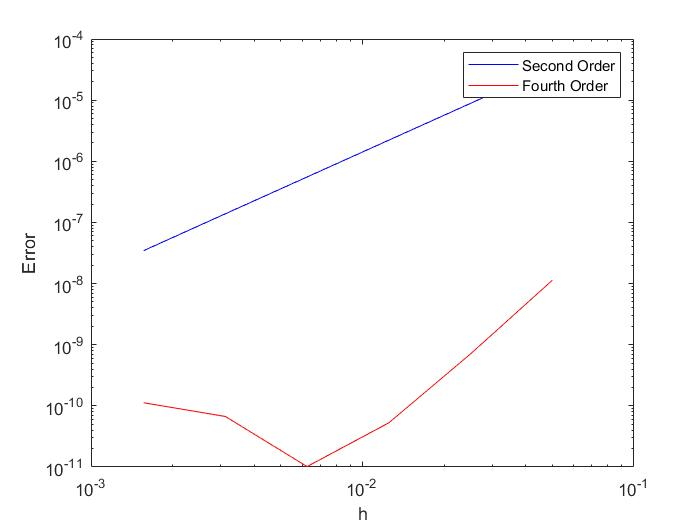
\includegraphics[width=10cm]{24.jpg} 
 \end{center}
 
 \item
 Since we expect that $F_2(h)$ generate an error of second order, and $\dfrac{2^2\cdot F_2(h/2) - F_2(h)}{2^2-1}$, which generally generate $F_3(h)$, which has an error of third error, but due to the symmetry here, we can get an error of fourth order here. And the expected reduction factor of second order and forth order is that 
 
 \lstinputlisting[language=Matlab,caption={expected}]{expect.txt}
 
 And compared with the column of $redfac2$ and $redfac4$, we found that the $redfac4$ seems incorrect when $h<0.025$, and this may cause by the rounding error when we subtract two nearly same value, namely, since $h$ is small, so that $4\times F_2(x+h/2)$ and $F_2(x+h)$ are close, and cause a large rounding error, but we do not have a good remedy here, so we can examine it by change the scale of h, so when we set h to

 \begin{lstlisting}[language=Matlab,frame =none]
 hvec = 0.1 *0.9.^(1:6);
 \end{lstlisting} 
 And the expected reduction factor of second order and forth order is that 
 
 \lstinputlisting[language=Matlab,caption={expected\_0.9}]{expect9.txt}
 
 And our table output is 
 \begin{small}
 \lstinputlisting[language=Matlab,caption={output\_0.9}]{output9.txt}
 \end{small}
 which support my expectation, and we can observe that of the graph, which is 
  \begin{center}
  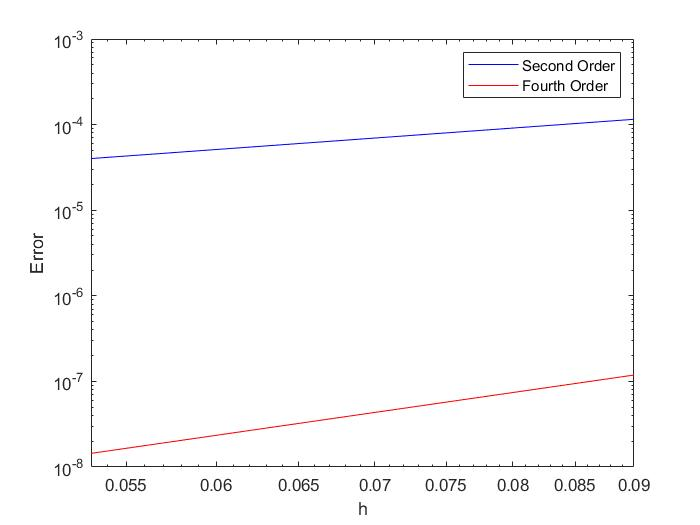
\includegraphics[width=10cm]{24_9.jpg} 
 \end{center}
 we can observe that the graph make more sense that when h decreases, the error always decreases, and when error is in second order, we know that \begin{align*}
 e2 &=O(h^2)\\
 \ln(e2)&=2 \ln(h) +c\\
  e4 &=O(h^4)\\
 \ln(e4)&=4 \ln(h) +c
\end{align*}  
 and the slope approximate shows the pattern of $+2$ and $+4$ respectively.
 
  Thus the $F_4$ here actually exhibit an error of forth order.
\end{enumerate}
\item
\begin{enumerate}
\item
\begin{align*}
\int_0^2 x\cos(x) dx &= \int_{x=0}^2 x d\sin(x)\\
&= x\sin(x)|_{x=0}^2 -\int_{x=0}^2 \sin(x) dx\\
&=(2\sin(2)-0)+\cos(x)|_{x=0}^2\\
&=2\sin(2)+\cos(2)-1
\end{align*}
\begin{itemize}
\item  m =1
\begin{align*}
\int_{0}^2 x \cos(x) dx &\approx 2\cdot (f(0) +f(2)) /2\\
&=f(0)+f(2)\\
&=2\cos(2)\\
\end{align*}
And we can calculate the error is\begin{align*}
e &= |2\cos(2)-2\sin(2)-\cos(2)-1|\\
&= 2\sin(2) - \cos (2)-1\\
&\approx 1.23
\end{align*}
\item m=2
\begin{align*}
\int_{0}^2 x \cos(x) dx &\approx  (f(0) +2f(1)+f(2))/2\\
&=(f(0)+2f(1)+f(2))/2\\
&=(2\cos(1)+2\cos(2))/2\\
&=\cos(1)+\cos(2)
\end{align*}
And we can calculate the error is\begin{align*}
e &= |\cos(1)+\cos(2)-2\sin(2)-\cos(2)+1|\\
&= 2\sin(2) - \cos (1)-1\\
&\approx 0.28
\end{align*}
\item  m=4
\begin{align*}
\int_0^2 x\cos(x) dx &\approx \dfrac{1}{2}\cdot \dfrac{f(0)+2f(1/2)+2f(1)+2f(3/2)+f(2)}{2}\\
&=\dfrac{ \cos(1/2)+2\cdot \cos(1)+3\cdot \cos(3/2)+2\cos(2))}{4}\\
&=\dfrac{\cos(1/2)}{4}+\dfrac{\cos(1)}{2}+\dfrac{3\cdot \cos(3/2)}{4}+\dfrac{\cos(2)}{2}
\end{align*}
And we can calculate the error is\begin{align*}
e &= \Big|\dfrac{\cos(1/2)}{4}+\dfrac{\cos(1)}{2}+\dfrac{3\cdot \cos(3/2)}{4}+\dfrac{\cos(2)}{2}-2\sin(2)-\cos(2)+1\Big|\\
&\approx 0.068
\end{align*}
\end{itemize}
\item
\begin{align*}
\int_0^1 \dfrac{1}{1+x^2} dx&=\int_0^1\dfrac{1}{1+tan^2\theta} d \tan\theta\\
&=\int_0^1\dfrac{\sec^2\theta}{1+tan^2\theta} d \theta\\
&=\int_0^1\dfrac{\sec^2\theta}{1+\frac{\sin^2\theta}{\cos^2\theta}} d \theta\\
&=\int_0^1\dfrac{1}{\cos^2\theta+{\sin^2\theta}} d \theta\\
&=\theta|_{x=0}^1\\
&=\arctan x|_0^1\\
&=\dfrac{\pi}{4}
\end{align*}
\begin{itemize}
\item  m =1
\begin{align*}
\int_0^1 \dfrac{1}{1+x^2} dx&\approx 1\cdot \dfrac{f(0)+f(1)}{2}\\
&=\dfrac{1+\frac{1}{2}}{2}\\
&=\dfrac{3}{4}
\end{align*}
And the error is \begin{align*}
e&=\Big|\dfrac{3}{4}-\dfrac{\pi}{4}\Big|\\
&\approx 0.035
\end{align*}
\item m=2
\begin{align*}
\int_0^1 \dfrac{1}{1+x^2} dx&\approx \dfrac{1}{2}\cdot \dfrac{f(0)+2f(1/2)+f(1)}{2}\\
&=\dfrac{1+\frac{2}{1+1/4}+1/2}{4}\\
&=\dfrac{1+\frac{8}{5}+1/2}{4}\\
&=\dfrac{31}{40}
\end{align*}
And the error is
\begin{align*}
e&=\Big|\dfrac{31}{40}-\dfrac{\pi}{4}\Big|\\
&\approx 0.0104
\end{align*}
\item  m=4
\begin{align*}
\int_0^1 \dfrac{1}{1+x^2} dx&\approx \dfrac{1}{4}\dfrac{f(0)+2f(1/4)+2f(1/2)+2f(3/4)+f(1)}{2}\\
&=\dfrac{1+\dfrac{2}{1+1/16}+\dfrac{2}{1+1/4}+\dfrac{2}{1+9/16}+1/2}{8}\\
&=\dfrac{5323}{6800}
\end{align*}
And the error is
\begin{align*}
e&=\Big|\dfrac{5323}{6800}-\dfrac{\pi}{4}\Big|\\
&\approx 0.002604
\end{align*}
\end{itemize}
\end{enumerate}
\item
\begin{enumerate}
\item
\begin{align*}
\int_0^2 \dfrac{dx}{\sqrt{2-x}}&=\int_0^2 (2-x)^{-1/2}dx\\
&=-\int_0^2 (2-x)^{-1/2}d(2-x)\\
&=-2(2-x)^{1/2}|_{x=0}^2\\
&=2\sqrt{2}
\end{align*}
\begin{itemize}
\item  m =1

\begin{align*}
\int_0^2 \dfrac{dx}{\sqrt{2-x}}&\approx 2f(1)\\
&=2\cdot\dfrac{1}{\sqrt{2-1}}\\
&=2
\end{align*}
And the error is \begin{align*}
e&=|2-2\sqrt{2}|\\
&=2(\sqrt{2}-1)\\
&\approx 0.828
\end{align*}
\item m=2
\begin{align*}
\int_0^2 \dfrac{dx}{\sqrt{2-x}}&\approx f(1/2)+f(3/2)\\
&=\dfrac{1}{\sqrt{2-1/2}}+\dfrac{1}{\sqrt{2-3/2}}\\
&=\dfrac{1}{\sqrt{3/2}}+\dfrac{1}{\sqrt{1/2}}\\
&=\sqrt{2/3}+\sqrt{2}\\
&=\left(\dfrac{\sqrt{3}}{3}+1\right)\sqrt{2}
\end{align*}
And the error is \begin{align*}
e&=|\sqrt{2/3}+\sqrt{2}-2\sqrt{2}|\\
&=|\sqrt{2/3}-\sqrt{2}|\\
&\approx 0.598
\end{align*}
\item  m=4
\begin{align*}
\int_0^2 \dfrac{dx}{\sqrt{2-x}}&\approx \dfrac{1}{2}(f(1/4)+f(3/4)+f(5/4)+f(7/4))\\
&=\dfrac{1}{2}\left(\dfrac{1}{\sqrt{2-1/4}}+\dfrac{1}{\sqrt{2-3/4}}+\dfrac{1}{\sqrt{2-5/4}}+\dfrac{1}{\sqrt{2-7/4}}\right)\\
&=\dfrac{1}{2}\left(\dfrac{1}{\sqrt{7/4}}+\dfrac{1}{\sqrt{5/4}}+\dfrac{1}{\sqrt{3/4}}+\dfrac{1}{\sqrt{1/4}}\right)\\
&=\dfrac{1}{2}\left(\sqrt{4/7}+{\sqrt{4/5}}+{\sqrt{4/3}}+{\sqrt{4}}\right)\\
&=\sqrt{1/7}+{\sqrt{1/5}}+{\sqrt{1/3}}+1\\
\end{align*}
And the error is \begin{align*}
e&=|\sqrt{1/7}+{\sqrt{1/5}}+{\sqrt{1/3}}+1-2\sqrt{2}|\\
&\approx 0.426
\end{align*}
\end{itemize}
\item
\begin{itemize}
\item  m =1
\begin{align*}
\int_0^{\pi/2} \dfrac{\cos(x)}{\pi/2-x} dx&\approx \pi/2 f(\pi/4)\\
&=\pi/2\cdot\dfrac{\cos(\pi/4)}{\pi/4}\\
&=2\cos(\pi/4)\\
&=\sqrt{2}
\end{align*}
\item m=2
\begin{align*}
\int_0^{\pi/2} \dfrac{\cos(x)}{\pi/2-x} dx&\approx \pi/4 (f(\pi/8)+f(3\pi/8))\\
&=\pi/4\cdot\left(\dfrac{\cos(\pi/8)}{3\pi/8}+\dfrac{\cos(3\pi/8)}{\pi/8}\right)\\
&=\dfrac{\cos(\pi/8)}{3/2}+\dfrac{\cos(3\pi/8)}{1/2}\\
&=\dfrac{\sqrt{\sqrt{2}+2}}{3}+\sqrt{2-\sqrt{2}}
\end{align*}
\item  m=4
\begin{align*}
\int_0^{\pi/2} \dfrac{\cos(x)}{\pi/2-x} dx&\approx \pi/8 (f(\pi/16)+f(3\pi/16)+f(5\pi/16)+f(7\pi/16))\\
&=\pi/8\cdot\left(\dfrac{\cos(\pi/16)}{7\pi/16}+\dfrac{\cos(3\pi/16)}{5\pi/16}+\dfrac{\cos(5\pi/16)}{3\pi/16}+\dfrac{\cos(7\pi/16)}{\pi/16}\right)\\
&=\dfrac{\cos(\pi/16)}{7/2}+\dfrac{\cos(3\pi/16)}{5/2}+\dfrac{\cos(5\pi/16)}{3/2}+\dfrac{\cos(7\pi/16)}{1/2}
\end{align*}
\end{itemize}
\end{enumerate}
\item
\begin{itemize}
\item  $f(x) =1$

\begin{align*}
LHS &=\int_{x_0}^{x_4} 1 dx\\
&=x_4-x_0\\
RHS &=\dfrac{2h}{45}(7+32+12+32+7)\\
&=4h\\
&=x_4-x_0\\&=LHS
\end{align*}


\item  $f(x) =x$

\begin{align*}
LHS &=\int_{x_0}^{x_4} x dx\\
&=\dfrac{1}{2} x^2|_{x_0}^{x_4}\\
&=\dfrac{x_4^2 - x_0^2}{2}\\ 
&=\dfrac{(x_4 - x_0)(x_4+x_0)}{2}\\ 
&=\dfrac{4h(x_0+4h+x_0)}{2}\\ 
&=2h(2x_0+4h)\\
&=4hx_0+8h^2\\
\end{align*}
\begin{align*}
RHS &=\dfrac{2h}{45}(7x_0+32x_1+12x_2+32x_3+7x_4)\\
&=\dfrac{2h}{45}(7x_0+32(x_0+h)+12(x_0+2h)+32(x_0+3h)+7(x_0+4h))\\
&=\dfrac{2h}{45}(90x_0+180h)\\
&=4hx_0+8h^2\\&=LHS
\end{align*}
\item $f(x) =x^2$
\begin{align*}
LHS &=\dfrac{x^3}{3}|_{x_0}^{x_4}\\
&=\dfrac{x_4^3-x_0^3}{3}\\
&=\dfrac{(x_4-x_0)(x_4^2+x_4x_0+x_0^2)}{3}\\
&=\dfrac{4h((x_0+4h)^2+(x_0+4h)\cdot x_0+x_0^2)}{3}\\
&=\dfrac{4h(x_0^2+8x_0h+16h^2+x_0^2+4hx_0+x_0^2)}{3}\\
&=\dfrac{4h}{3}(3x_0^2+12x_0h+16h^2)\\
\end{align*}
\begin{align*}
RHS &=\dfrac{2h}{45}(7x_0^2+32x_1^2+12x_2^2+32x_3^2+7x_4^2)\\
&=\dfrac{2h}{45}(7x_0^2+32(x_0+h)^2+12(x_0+2h)^2+32(x_0+3h)^2+7(x_0+4h)^2)\\
&=\dfrac{2h}{45}(90x_0^2+360x_0h+480h^2)\\
&=4x_0^2h+16x_0h^2+\dfrac{64 h^3}{3}\\
&=\dfrac{4h}{3}(3x_0^2+12x_0h+16h^2)\\&=LHS
\end{align*}
\item $f(x) = x^3$
\begin{align*}
LHS &=\dfrac{x^4}{4}|_{x_0}^{x_4}\\
&=\dfrac{x_4^4-x_0^4}{4}\\
&=\dfrac{(x_4-x_0)(x_4+x_0)(x_4^2+x_0^2)}{4}\\
&=\dfrac{4h(2x_0+4h)(x_0^2+(x_0+4h)^2)}{4}\\
&=h(2x_0+4h)(x_0^2+x_0^2+8hx_0+16h^2)\\
&=2h(2x_0+4h)(x_0^2+4hx_0+8h^2)\\
&=4h(x_0+2h)(x_0^2+4hx_0+8h^2)\\
&=4h(x_0^3+4hx_0^2+8h^2x_0+2hx_0^2+8h^2x_0+16h^3)\\
&=4h(x_0^3+6hx_0^2+16h^2x_0+16h^3)\\
\end{align*}
\begin{align*}
RHS &=\dfrac{2h}{45}(7x_0^3+32x_1^3+12x_2^3+32x_3^3+7x_4^3)\\
&=\dfrac{2h}{45}(7x_0^2+32(x_0+h)^3+12(x_0+2h)^3+32(x_0+3h)^3+7(x_0+4h)^3)\\
&=\dfrac{2h}{45}(90x_0^3+540x_0^2h+1440x_0h^2+1440h^3)\\
&=4h(x_0^3+6x_0^2h+16x_0h^2+16h^3)\\&=LHS
\end{align*}
\item $f(x) = x^4$
\begin{align*}
LHS &=\dfrac{x^5}{5}|_{x_0}^{x_4}\\
&=\dfrac{(x_4 - x_0) (x_4^4 + x_4^3 x_0 + x_4^2 x_0^2 + x_4 x_0^3 + x_0^4)}{5}\\
&=\dfrac{4h}{5}(5x_0^4+40x_0^3h+160x_0^2h^2+320x_0h^3+256h^4)
\end{align*}
\begin{align*}
RHS &=\dfrac{2h}{45}(7x_0^4+32x_1^4+12x_2^4+32x_3^4+7x_4^4)\\
&=\dfrac{2h}{45}(7x_0^4+32(x_0+h)^4+12(x_0+2h)^4+32(x_0+3h)^4+7(x_0+4h)^4)\\
&=\dfrac{2h}{45}(90x_0^4+720x_0^3h+2880x_0^2h^2+5760x_0h^3+4608h^4)\\
&=\dfrac{4h}{5}(5x_0^4+40x_0^3h+160x_0^2h^2+320x_0h^3+256h^4)\\&=LHS
\end{align*}
\item $f(x) = x^5$
\begin{align*}
LHS &=\dfrac{x^6}{6}|_{x_0}^{x_4}\\
&=\dfrac{(x_0 - x_4) (x_0 + x_4) (x_0^2 - x_4 x_0 + x_4^2) (x_0^2 + x_4 x_0 + x_4^2)}{6}\\
&=\dfrac{4h}{6}(1024 h^5 + 1536 x_0h^4 + 960 x_0^2h^3 + 320 x_0^3h^2 + 60 x_0^4h + 6x_0^5)\\
&=\dfrac{2h}{3}(1024 h^5 + 1536 x_0h^4 + 960 x_0^2h^3 + 320 x_0^3h^2 + 60 x_0^4h + 6x_0^5)
\end{align*}\begin{align*}
RHS &=\dfrac{2h}{45}(7x_0^5+32x_1^5+12x_2^5+32x_3^5+7x_4^5)\\
&=\dfrac{2h}{45}(7x_0^5+32(x_0+h)^5+12(x_0+2h)^5+32(x_0+3h)^5+7(x_0+4h)^5)\\
&=\dfrac{2h}{45}(15360 h^5 + 23040 x_0h^4 + 14400 x_0^2h^3 + 4800 x_0^3h^2 + 900 x_0^4h + 90x_0^5)\\
&=\dfrac{2h}{3}(1024 h^5 + 1536 x_0h^4 + 960 x_0^2h^3 + 320 x_0^3h^2 + 60 x_0^4h + 6x_0^5)\\&=LHS
\end{align*}
\item $f(x) = x^6$
\begin{align*}
LHS &=\dfrac{x^7}{7}|_{x_0}^{x_4}\\
&=\dfrac{-(x_0 - x_4) (x_0^6 + x_4 x_0^5 + x_4^2 x_0^4 + x_4^3 x_0^3 + x_4^4 x_0^2 + x_4^5 x_0 + x_4^6)}{7}\\
&=\dfrac{4h}{7}(4096 h^6 + 7168 h^5 x_0 + 5376 h^4 x_0^2 + 2240 h^3 x_0^3 + 560 h^2 x_0^4 + 84 h x_0^5 + 7 x_0^6)\\
&=4h\left( \dfrac{4096}{7} h^6 + 1024 h^5 x_0 + 768 h^4 x_0^2 + 320 h^3 x_0^3 + 80 h^2 x_0^4 + 12 h x_0^5 + x_0^6\right)
\end{align*}
\begin{align*}
RHS &=\dfrac{2h}{45}(7x_0^6+32x_1^6+12x_2^6+32x_3^6+7x_4^6)\\
&=\dfrac{2h}{45}(7x_0^6+32(x_0+h)^6+12(x_0+2h)^6+32(x_0+3h)^6+7(x_0+4h)^6)\\
&=\dfrac{2h}{45}(52800 h^6 + 92160 h^5 x_0 + 69120 h^4 x_0^2 + 28800 h^3 x_0^3 + 7200 h^2 x_0^4 + 1080 h x_0^5 + 90 x_0^6)\\
&=4h\left(\dfrac{1760 h^6}{3} + 1024 h^5 x_0 + 768 h^4 x_0^2 + 320 h^3 x_0^3 + 80 h^2 x_0^4 + 12 h x_0^5 + x_0^6\right)\\
\because \dfrac{4096}{7}&\neq \dfrac{1760}{3}\\
\therefore RHS&\neq LHS
\end{align*}
\end{itemize}
Therefore, the degree of precision is 5.

 \end{enumerate}
\end{document}